
%(BEGIN_QUESTION)
% Copyright 2010, Tony R. Kuphaldt, released under the Creative Commons Attribution License (v 1.0)
% This means you may do almost anything with this work of mine, so long as you give me proper credit

Read and outline the ``Sequencers'' subsection of the ``Ladder Diagram (LD) Programming'' section of the ``Programmable Logic Controllers'' chapter in your {\it Lessons In Industrial Instrumentation} textbook.  Note the page numbers where important illustrations, photographs, equations, tables, and other relevant details are found.  Prepare to thoughtfully discuss with your instructor and classmates the concepts and examples explored in this reading.

\vskip 20pt \vbox{\hrule \hbox{\strut \vrule{} {\bf Suggestions for Socratic discussion} \vrule} \hrule}

\begin{itemize}
\item{} If you have access to your own PLC for experimentation, I urge you to write a simple {\it demonstration} program in your PLC allowing you to explore the behavior of these PLC instructions.  The program doesn't have to do anything useful, but merely demonstrate what each instruction does.  First, read the appropriate section in your PLC's manual or instruction reference to identify the proper syntax for that instruction (e.g. which types of data it uses, what address ranges are appropriate), then write the simplest program you can think of to demonstrate that function in isolation.  Download this program to your PLC, then run it and observe how it functions ``live'' by noting the color highlighting in your editing program's display and/or the numerical values manipulated by each instruction.  After ``playing'' with your demonstration program and observing its behavior, write comments for each rung of your program explaining in your own words what each instruction does.
\end{itemize}

\underbar{file i04529}
%(END_QUESTION)





%(BEGIN_ANSWER)


%(END_ANSWER)





%(BEGIN_NOTES)

Drum sequencer mechanisms worked like a ``player piano'' to actuate a set of electrical switches according to a timed schedule and/or a sequence of discrete events.  CIP (Clean In Place) sequences for cleaning food processing vessels is one application for drum sequencers (rinse, caustic, acid, rinse).  Burner management systems for starting combustion processes is another application for drum sequencers (purge, wait, ignition, monitor).

\vskip 10pt

Drum sequencers are a type of state machine, where the output of the device depends not only on present input conditions but also the internal state of the device which is influenced by past input conditions as well.  PLCs can easily perform sequencing functions, but unfortunately there is little standardization among PLC manufacturers for programming these functions.

\vskip 10pt

Koyo PLCs use a ``drum'' instruction showing the on/off states as colored squares inside a larger box, somewhat resembling a mechanical drum sequencer.  Columns represent different output bits, while rows represent steps in the sequence.  Drum instructions may be time-based or event-based (i.e. the condition necessary to advance to the next step might simply be a time delay, or may alternatively be an input event which needs to take place).

$$\includegraphics[width=15.5cm]{i04529x01.eps}$$

\filbreak

$$\includegraphics[width=15.5cm]{i04529x02.eps}$$

\vskip 10pt

Allen-Bradley sequencer instructions are much more sophisticated.  The SQO instruction steps through a set of pre-loaded bit registers in memory (typically {\tt B3} registers) not represented visually in the instruction like the Koyo drum instruction.  In the Koyo drum, the bit states for each step are a fixed parameter of the instruction, set at programming time.  In the Allen-Bradley SQO instruction, the bit states may be altered during run time, as the referenced bits are simply {\tt B3} registers, which may be altered dynamically like any other area of memory.  Also, the Allen-Bradley SQO instruction has the ability to read from any area of the PLC's memory, not just bits like the Koyo drum instruction.  This makes it possible for an SQO instruction to read integer numbers, ASCII text characters, etc. at each step of the programmed sequence.

$$\includegraphics[width=15.5cm]{i04529x03.eps}$$

An indexed address is given in the ``File'' parameter, showing the starting address in memory when the SQO instruction's ``Position'' variable is zero.  As the Position increments, the next address following the indexed reference will be read by the SQO instruction (i.e. if File = {\tt \#B3:0}, then {\tt B3:0} will be read when Position = 0; {\tt B3:1} will be read when Position = 1; etc.).  The Mask parameter tells the SQO instruction which bits in the 16-bit word will be written to the Output file.  The Mask parameter functions analogously to masking tape, declaring only a certain range of bits to be ``painted'' by the SQO instruction.

SQO instructions are fundamentally event-driven, the instruction proceeding to the next position when the input transitions from false to true (from off to on).

\vskip 10pt

Two SQO instructions may be used in tandem with a timer to form a time-based sequencing program: one SQO instruction reads control bits to be output by the PLC, while the other SQO instruction reads time values stored in {\tt N7} registers to preload the timer, thus setting the time duration of each step in the sequence.

\vskip 10pt

An SQO instruction may be used in tandem with an SQC instruction to form an event-based sequencing program: the SQC instruction compares the contents of an indexed register against a Source file, setting a ``Found'' ({\tt /FD}) bit when the two match.  This ``Found'' bit may then be used to advance both SQO and SQC instructions to the next position.

\vskip 10pt

The Allen-Bradley SQL instruction loads data into a series of indexed registers, allowing the PLC to dynamically input data according to a sequenced schedule.  This is useful for datalogging, where live input data may be stored in memory registers at certain intervals of time or of events.  There is no analogue in the Koyo PLCs to this function!








\vskip 20pt \vbox{\hrule \hbox{\strut \vrule{} {\bf Suggestions for Socratic discussion} \vrule} \hrule}

\begin{itemize}
\item{} Give at least one practical example of a drum sequencer in an industrial process.
\item{} Explain the difference between a {\it time}-based drum sequencer and an {\it event}-based drum sequencer.
\item{} Explain the function of the {\it mask} parameter in an Allen-Bradley SQO instruction.
\end{itemize}

%INDEX% Reading assignment: Lessons In Industrial Instrumentation, Programmable Logic Controllers (sequencers)

%(END_NOTES)

